\chapter{相关技术介绍}
基于神经网络的分布表示一般称为词向量、词嵌入(Word Embedding)或分布式表示(Distributed Representation)~\upcite{DBLP:conf/nips/MikolovSCCD13}。神经网络词向量表示技术通过神经网络技术对上下文(Context),以及上下文与目标词之间的关系进行建模。由于神经网络较为灵活,这类方法的最大优势在于可以表示复杂的上下文。在前面基于矩阵的分布表示方法中,最常用的上下文是词。如果使用包含词序信息的n-gram 作为上下文,当n 增加时,n-gram 的总数会呈指数级增长,此时会遇到维数灾难问题。而神经网络在表示n-gram 时,可以通过一些组合方式对n 个词进行组合,参数个数仅以线性速度增长。有了这一优势,神经网络模型可以对更复杂的上下文进行建模,在词向量中包含更丰富的语义信息。神经网络模型主要包括: 传统前向传递神经网络(Feed Forward Neural Network, FFNN)、循环神经网络(Recurrent Neural Network, RNN)建模方案。

另外针对大词表问题,主要可以分为以下两种策略:基于类别的多元分类模型(class-based hierarchical softmax, cHSM)和基于二叉树的二元分类模型(class-based hierarchical softmax,tHSM),我们分别在下面详细讨论和介绍。

\section{循环神经网络语言模型}
在这一节中,我们从语言模型任务的形式化开始,阐述语言模型的目标和应用~\upcite{DBLP:journals/tnn/ChienK16}。 具体来说,给定一个$T$个字的序列:$w_1,w_2,\cdots,w_T$,这个序列的对数概率(Log-probability),学习它的流畅性(Fluency)概率和相对似然性(Log Likelihood),可以被分解成一系列的条件概率 使用马尔可夫链规则:
\begin{equation}
\label{laguage_model}
 \log p(w_1,\cdots, w_T ) = \sum_{t=1}^T \log p(w_t | w_{1:t-1}),
\end{equation}
其中前 $t-1$个单词记作$w_ {1:t-1}$。进而,条件概率~$p(w_t | w_ {1:t-1})$表示给定其前面上下文$ w_1,\cdots,w_ {t-1} $作为输入的下一个单词的条件概率(Conditional Probability), 传统上由前馈网络建模~\upcite{DBLP:journals/jmlr/BengioDVJ03}。 训练整个模型以最小化每个时间步的交叉熵损失(Cross Entropy Loss):
\begin{equation}\label{equ:losses}
  \ell=\sum_{t=1}^{T}\ell_t=\sum_{t=1}^{T}\log p(w_t | w_{1:t-1})
\end{equation}
其中交叉熵是由KL散度(Kullback–Leibler Divergence),也叫做相对熵(Relative Entropy),推导而获得的。需要注意的是,交叉熵的定义是当编码方案不一定完美时(由于对概率分布的估计不一定正确),平均编码长度的是多少。
\begin{equation}\label{equ:losses}
  KL(p||q)=-\sum_{t=1}^{T}p(x)\log q(x) - (\sum_{t=1}^{T}p(x)\log p(x))
\end{equation}
其中$p(x)$ 是数据的真实概率分布,$q(x)$ 是由数据计算得到的概率分布。需要注意的是,由于$p(x)$ 和$q(x)$ 在公式中的地位不是相等的,所以$\tt KL \it(p\parallel q)\not\equiv \tt KL \it (q\parallel p)$。对于特定的训练数据集,第二项的计算值是常数,由此可知其导数是0,不会对参数更新产生任何影响,所以通常情况下,我们采用交叉熵函数作为模型的代价函数,但其实我们希望模型优化的目标是使得模型的分布拟合实际的分布。

最近,利用序列的时间序列信息的循环神经网络已经非常流行,如图~\ref{fig:lm}~所示。 为了清楚起见,由于在当前时间步 $ t $的输出$ w_ {t + 1} $正好是下一个时间步的输入$ w_ {t + 1} $,所以没有输出的自动关联连接 的前一次步骤$ t $回到下一个时间步骤$ t + 1 $中的递归神经网络。

如图~\ref{fig:lm} 所示,每个句子都需要用开始词(即,$ \langle s \rangle $)和结束词(即$ \langle / s \rangle $)标记进行封装。 在预测下一个单词 $ w_ {t + 1} $ 之前,从最后一个隐藏状态$ h_ {t-1} $和当前字$ w_t $接收到循环网络单元的输入。
\begin{figure}[!ht]
  \centering
  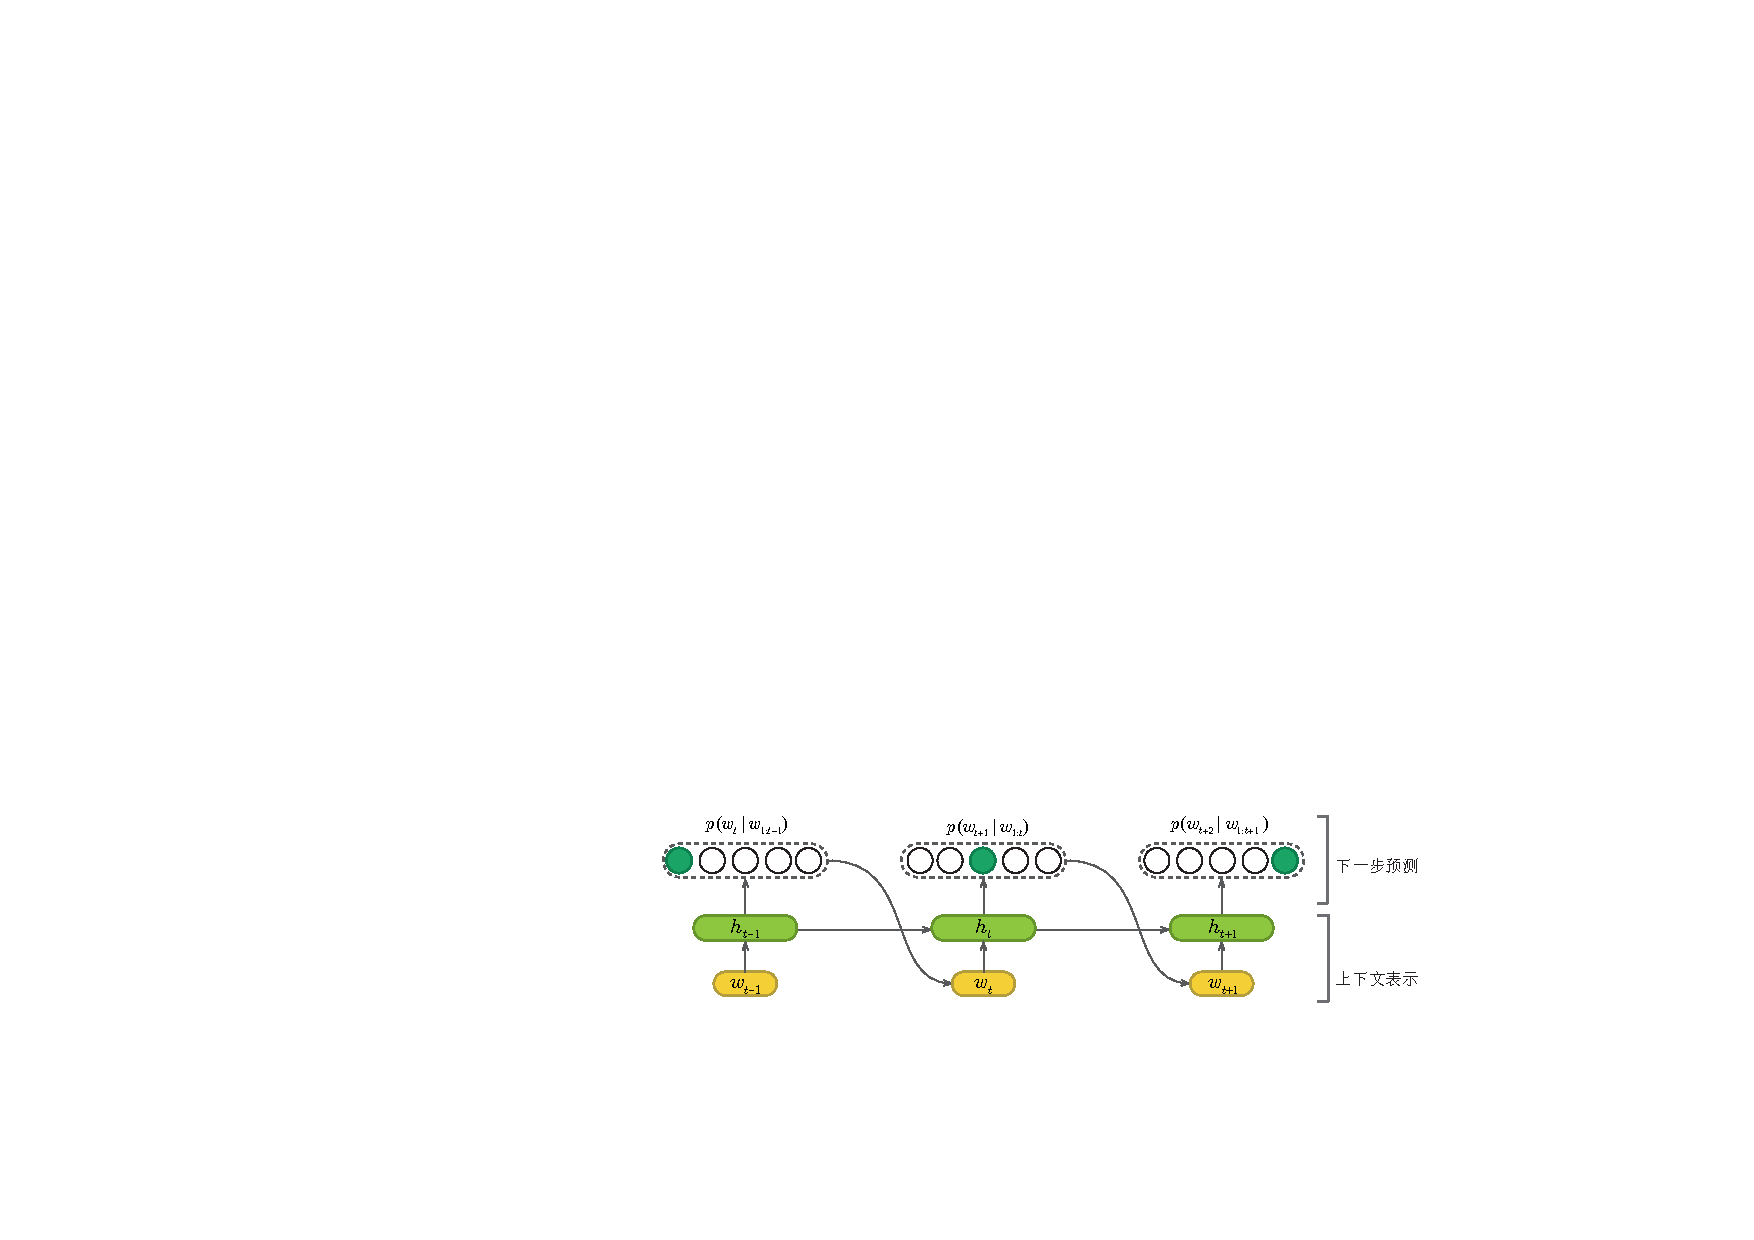
\includegraphics[width=1\columnwidth]{./figures/lm.pdf}
  \caption{循环神经网络语言模型图例}
  \label{fig:lm}
\end{figure}

从形式上讲,循环神经网络是一个参数化的非线性函数$ \mathtt{RNN} $,循环地将一系列向量映射到一系列隐藏状态。 将$ \mathtt{RNN} $应用于任何这样的序列,在每个时间步骤$ t $产生隐藏状态$ h_t $,如下所示:
\begin{equation}
  h_t \leftarrow  \mathtt{RNN}(W\theta^w_t + U h_{t-1} +c),
\end{equation}
其中$ W,U $是模型参数的集合,而$ U $是随时间共享的,向量$ \theta^w_t$ 对应于源词的嵌入$ w_t $。

自Elman提出基本循环网络模型~\upcite{DBLP:journals/cogsci/Elman90}~以来,已经有许多扩展模型提出了克服长距离依赖,梯度消失(Gradient Vanishing)和梯度爆炸(Gradient Exploding)等问题, 如长期短期记忆网络(LSTM)~\upcite{7508408},门限记忆单元(GRU)~\upcite{DBLP:conf/nips/ChungKDGCB15}和近似递归神经网络(Quasi-RNNs)\upcite{DBLP:journals/corr/BradburyMXS16}。

\subsection{长距离短期记忆网络}
 LSTM的计算公式定于如下 \upcite{DBLP:journals/neco/HochreiterS97}:
\begin{itemize}
\item 输入门。控制当前输入 $x_t$ 和前一步输出 $h_{t−1}$ 进入新的 cell 的信息量:$i_t=\sigma(W^i x_t+U^i h_{t-1}+b^i)$
\item  遗忘门。决定是否清楚或者保持单一部分的状态$f_t=\sigma(W^f x_t+U^f h_{t-1}+b^f)$
\item  变换输出和前一状态到最新状态$g_t=\phi(W^g x_t+U^g h_{t-1}+b^g)$
\item  输出门。计算 cell 的输出$o_t=\sigma(W^o x_t+U^o h^{t-1}+b^o)$
\item  cell 状态更新。步骤:计算下一个时间戳的状态使用经过门处理的前一状态和输入:$s_t=g_t\odot i_t+s_{t-1}\odot f_t$
\item 最终 LSTM 的输出:使用一个对当前状态的 $\tanh$ 变换进行重变换:$h_t=s_t\odot \phi(o_t)$
\end{itemize}
\noindent 其中$\odot$ 代表对应元素相乘(Element-wise Matrix Multiplication), 函数 $\phi(x), \sigma(x)$ 的定义如下:
\begin{equation}\label{equ:tanh}
  \phi(x)=\frac{e^x-e^{-x}}{e^x+e^{-x}},\sigma(x)=\frac{1}{1+e^{-x}}
\end{equation}

\begin{figure}
  \centering
  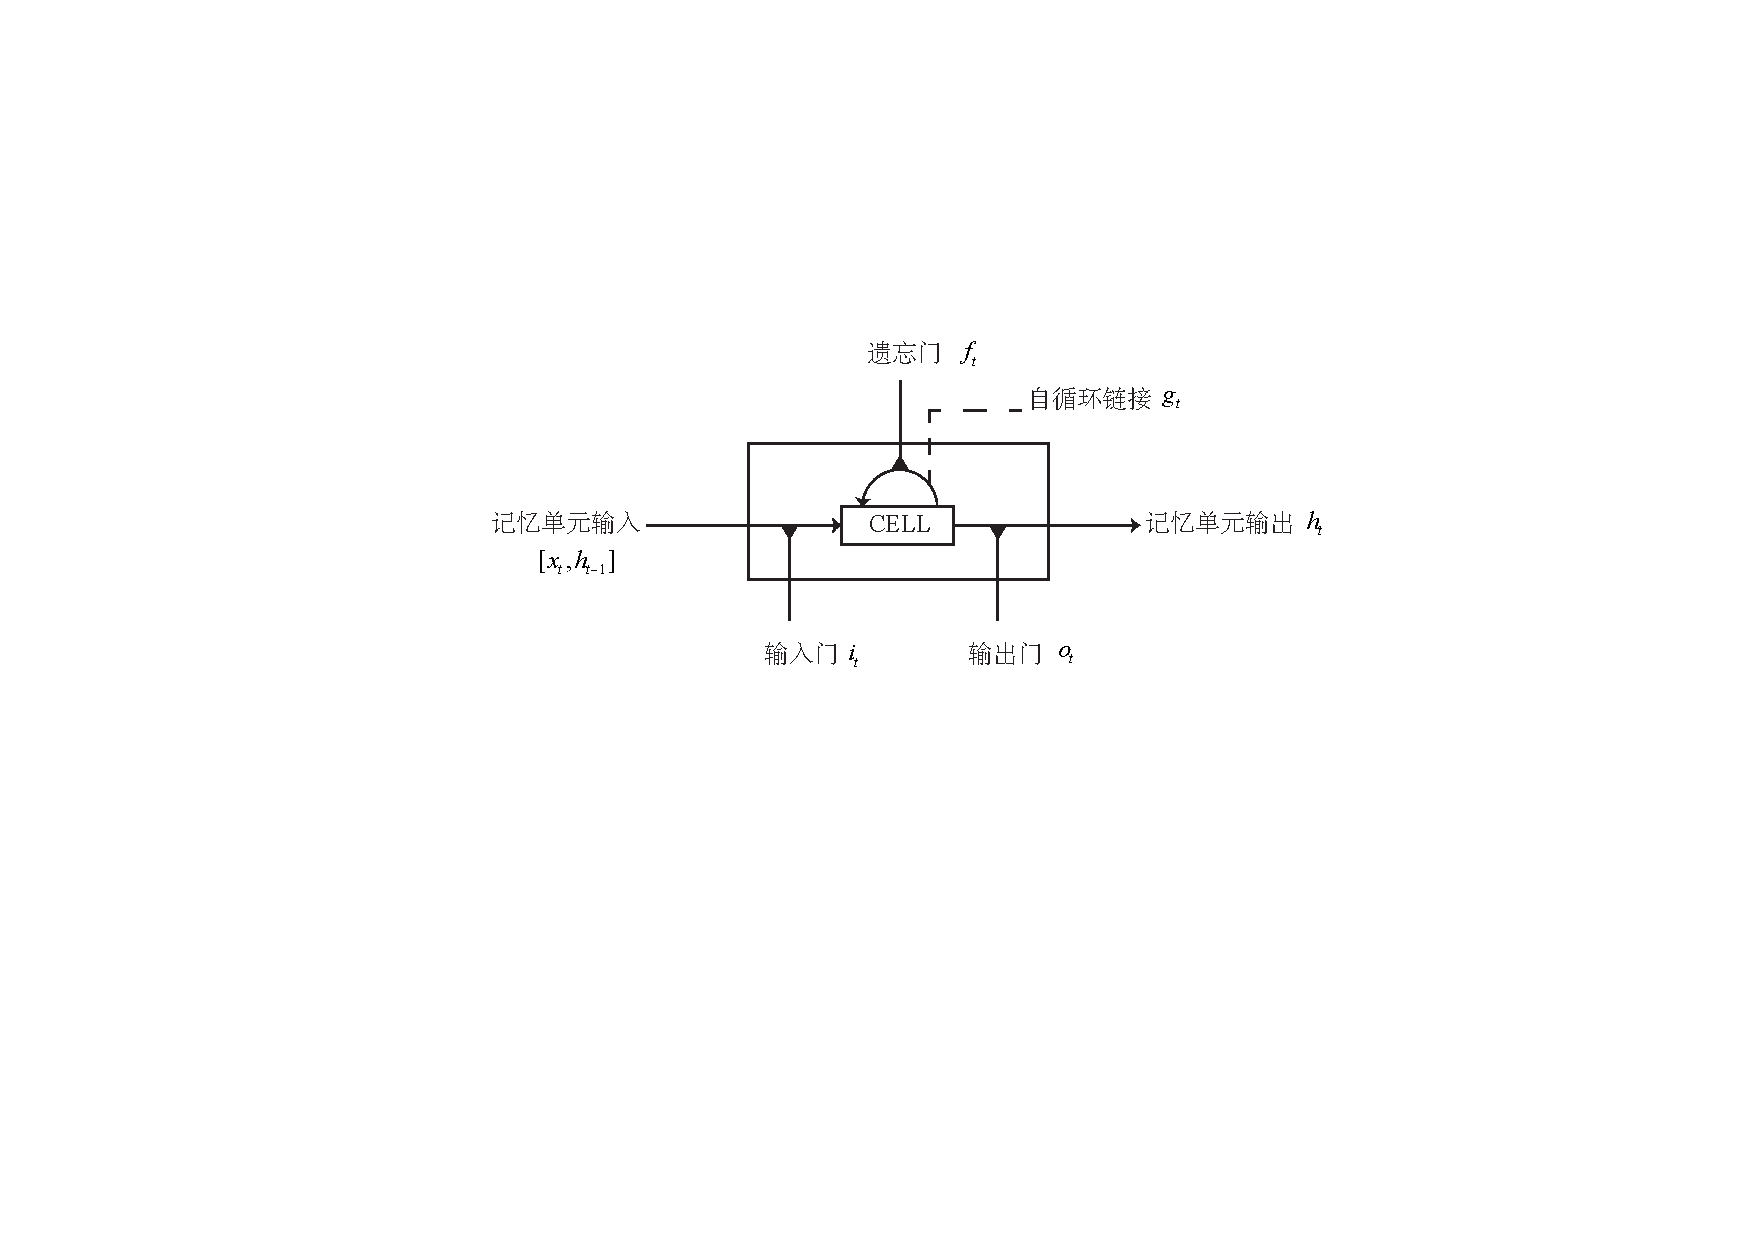
\includegraphics[width=0.7\linewidth]{./figures/lstm.pdf}
  \caption{LSTM 模型示意图}\label{fig:lstm}
\end{figure}

\subsection{门限记忆单元}
GRU 可以看成是 LSTM 的变种,GRU 把 LSTM中的 遗忘门和输入门用更新门来替代。 把 cell state 和隐状态 $h_t$ 进行合并,在计算当前时刻新信息的方法和 LSTM 有所不同。 下图是GRU更新 $h_t$ 的过程\upcite{DBLP:journals/corr/Pezeshki15}, 具体定义如下:
\begin{figure}[!h]
  \centering
  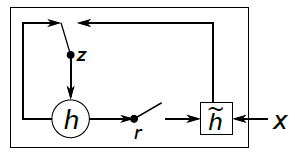
\includegraphics[width=0.45\linewidth]{./figures/gru.png}
  \caption{GRU模型示意图}\label{fig:gru}
\end{figure}

\begin{itemize}
\item 更新门 $z_t$。定义保存多少以前的信息: $z_t = \sigma ( W^z x_t+ U^z h_{t-1}  )$

\item 重置门 $r_t$。 决定保留多少输入信息: $r_t = \sigma(W^r x_t  + U^r h_{t-1}  )$

\item 节点内部更新值$\tilde h_t $。 其次是计算候选隐藏层(candidate hidden layer) $\tilde h_t$,这个候选隐藏层 和LSTM中的$\tilde c_t$是类似,可以看成是当前时刻的新信息,其中$r_t$用来控制需要 保留多少之前的记忆,如果$r_t$为0,那么$\tilde h_t$只包含当前词的信息:$\tilde h_t  = \tanh (W^h x_t  + U^h(h_{t-1} \odot r_t) )$

\item 隐藏层输出值$h_t$。 最后$z_t$控制需要从前一时刻的隐藏层 $h_{t-1}$ 中遗忘多少信息,需要加入多少当前 时刻的隐藏层信息$\tilde h_t$,最后得到$h_t$,直接得到最后输出的隐藏层信息, 这里与LSTM的区别是GRU中没有 输出门:$h_t = (1-z_t)\odot \tilde h_t  + z_t \odot h_{t-1}$
\end{itemize}

如果重置门接近0,那么之前的隐藏层信息就会丢弃,允许模型丢弃一些和未来无关 的信息;更新门 控制当前时刻的隐藏层输出$h_t$需要保留多少之前的隐藏层信息, 若$z_t$接近1相当于我们之前把之前的隐藏层信息拷贝到当前时刻,可以学习长距离依赖。 一般来说那些具有短距离依赖的单元重置门比较活跃(如果$r_t$为1,而$z_t$为$0$ 那么相当于变成了一个标准的RNN,能处理短距离依赖),具有长距离依赖的单元更新门比较活跃。



\section{大词表问题}
作为多标签分类(Multi-class Classification)的标准概率归一化方法,对于大词表优化而言,\texttt{log-softmax} 函数和相应的梯度可以定义为:
\begin{equation}
\label{eq:softmax}
\begin{split}
%p(w_i|h)=&\frac{\exp(h^\top v_{w_i})}{\sum_{w_j\in \mathcal{V}}{\exp(h^\top v_{w_j} )}} \\
\log p(w|h) &= \theta^w h-\log \sum_{u\in \mathcal{V}}{\exp(\theta^u h)}\\
%\frac{\partial p(w_i|h)}{\partial v_{w_j}}=&p(w_j|h)(\delta_{ij}-p(w_i|h))h^\top\\
\nabla_{\theta^u}{\log p(w|h)}&= (\delta_{uw}-p(w|h))h
\end{split}
\end{equation}
其中$ h $是隐藏层输出的向量(即上下文表示),$ \theta ^ w $表示单词$ w $的目标单词嵌入~\upcite{duda2012pattern}。 同样对于克罗内克 $\delta$ 函数$ \delta_ {uv} $(Kronecker Function),如果$ u,v $指代的是相同的单词结果是$ 1 $,如果不是相同的单词则是$ 0 $。


如等式~\ref{eq:softmax}~所示,前向概率传播函数(即第一行方程)和后向梯度优化函数(即第二行的方程)都需要计算目标词汇表中的所有单词,因此在这个部分上花费的时间会随着词汇量的增加而线性增长。对于包含$ \mathcal{| V |} $ 数量的单词来说,总的时间复杂度是$ \mathcal {O}(\mathcal {| H || V |})$,其中$ \mathcal {| H |} $表示隐藏层输出的维度。即使对于采用现代体系结构的GPU来说, 尽管其非常适合于具有高计算并行的矩阵乘法,这种计算负担也是相当高的。因此,在现代硬件体系结构的训练和推理中,输出字嵌入矩阵的超大尺寸仍然是一个计算瓶颈。

值得注意的是,\texttt{softmax} 算法的瓶颈不能归因于``for''循环函数(即方程~\ref{eq:softmax}~)中的$ \sum_ {u \in \mathcal {V}} $,尽管它随着词汇量的增长而线性增长,但是矩阵张量计算的规模较大。因为矩阵计算需要更多的时间来获得结果,但线性求和可以更快地计算完成。所以,相比于``for''循环函数而言,主要的计算时间用于矩阵乘法计算。在这里说明的目的是,只有那些避免其他冗余字的计算概率才能达到边际加速比的方法,而那些仍然涉及全局概率规一化的方法,实际上并不能真正改善这个部分的计算占用的时间。

%其中由于分母是正则项,一旦词表扩大,每次迭代更新都需要计算这一项,是主要的问题所在,所以本课题拟在主要解决该问题所导致的计算费时的问题,

因此,在保证计算精度不下降的情况下,我们期望能缓解计算概率归一化项的计算瓶颈并且提高模型的训练速度。 目前主要缓解大词表问题的算法主要分为以下三类: 单词拆分算法(Vocabulary Truncation)、采样估计模型(Sampling-based Approximation)和层次分解模型(Vocabulary Factorisation)。


\subsection{单词拆分算法}
针对大词表问题的解决方法,最直接最简单的策略就是我们放弃使用大词表,转而保留一个较小的词表来保证训练的内存占用小和计算效率高。那么针对剩余的过多的词表外的单词(Out-Of-Vocabulary,OOV),我们可以使用传统的N-gram语言模型来估算其可能的概率分布。这样做一方面保证神经网络模型可以在有限时间内训练完,同时保证模型的最后的测试结果不会很差~\upcite{DBLP:journals/csl/Schwenk07}。

然而我们需要注意到,当我们的词表继续减少和我们的所有单词种类不断变多的时候,我们会发现训练样本中存在过多的$\langle$unk$\rangle$ 字符,这样使得神经网络的模型训练非常困难,进而导致模型效果变得非常地差,所以这种方案只是一定程度上缓解了大词表问题,但是也是一种有效的尝试方案。

除了上述方案,目前采用的方案是将单词按照字符级别来划分,可以将一个单词按照字符统计规律划分成任意多个子词。其中二元对编码(byte-pair-encoding,BPE)能将一个单词划分成两部分:前缀(Prefix)和后缀(Suffix)~\upcite{DBLP:conf/icassp/Tucker0P94, DBLP:conf/acl/SennrichHB16a,Gage:1994:NAD:177910.177914},如图~\ref{fig:subword} 所示。由于划分规则是从训练数据中学习到的,我们可以指定需要缩减的词表大小,该算法的动态适应性很强,目前主流的机器翻译模型都采用这个方案~\upcite{DBLP:journals/corr/JozefowiczVSSW16}。尽管如此,我们仍然需要看到它这样的解构操作依然带来了一定的损失,因为句子的长度加倍了,对RNN的长距离关系学习能力提出了更高的挑战~\upcite{DBLP:conf/aaai/KimJSR16}。


如图~\ref{fig:subword}~所示,单词被划分成前缀和后缀两部分,其中$+$代表是单词的前缀,同时$\langle /w \rangle$是单词的后缀。
\begin{figure}[!h]
  \centering
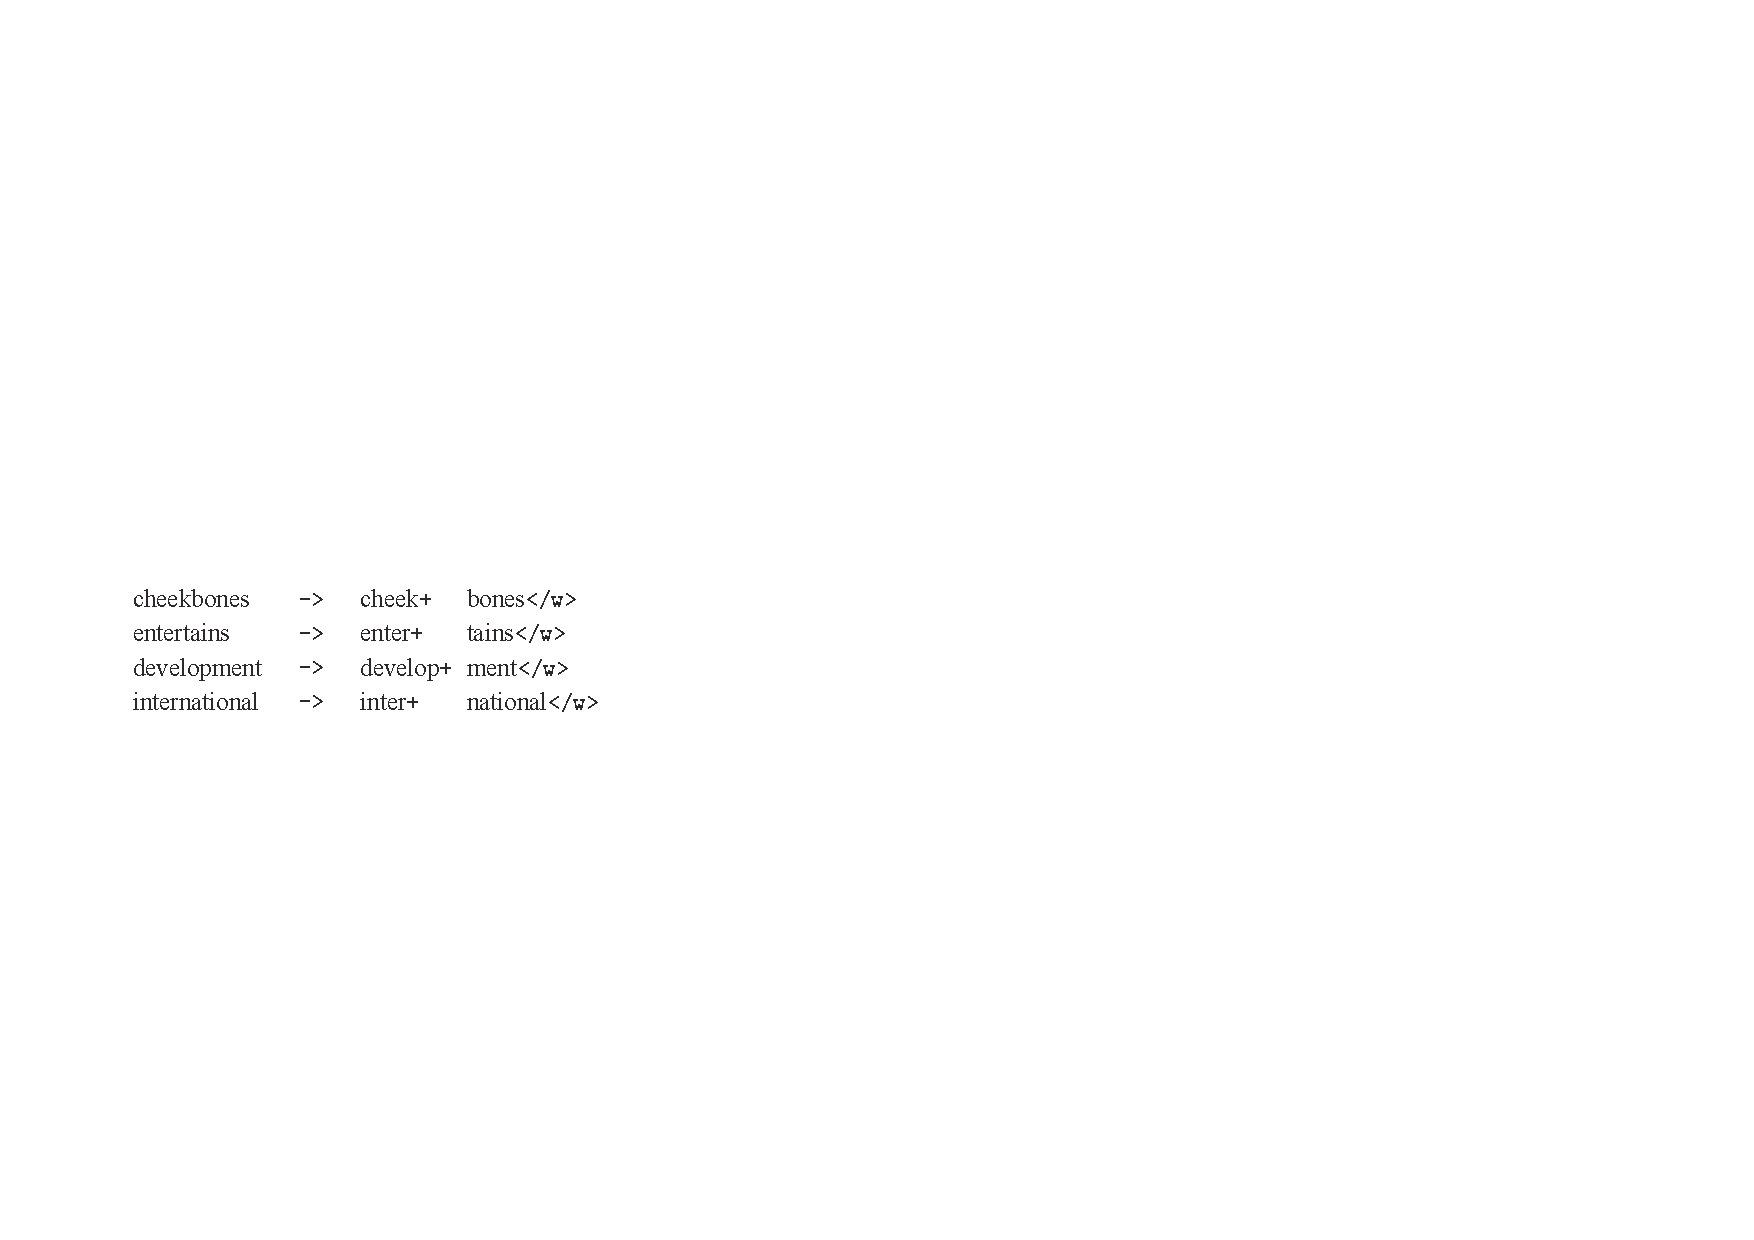
\includegraphics[width=0.6\linewidth]{./figures/subword.pdf}
\caption{词到子词划分样例}\label{fig:subword}
\end{figure}

\subsection{采样估计模型}
目前采用的采样算法(Sampling ALgorithm)主要是针对概率规约那一项进行概率估计,其中著名的算法有:重要性采样(Importance Sampling)~\upcite{DBLP:journals/tnn/BengioS08},噪声差分估计(Noise Contrastive Estimation, NCE)~\upcite{DBLP:conf/icml/MnihT12}和Blackout 采样算法~\upcite{DBLP:journals/iclr/JiVSAD15}。第一种算法在实验中被证明模型无法收敛,目前主要使用的后面两种算法。

对于NCE噪声差分估计算法来说,模型需要学习将正确的单词 $w_0$ 与随机生成的单词 $\{w_1\cdots w_k\}$做一个二元分类。 其中 $w_0$ 训练样本中真正的下一个单词, $\{w_1\cdots w_k\}$ 是采用先验分布  $q(w)$产生的随机噪声单词. 正例归一化后的概率和所有负例联合概率的公式可以写成:
\begin{equation}\label{equ:nce}
\begin{split}
  \tilde{p}(y=1|h)=&\frac{\exp( \theta^w_0 h)}{ \exp( \theta^w_0 h)+k *q(w_0)}\\
  \tilde{p}(y=0|h)=&\prod_{i=1}^{k}\frac{k *q(w_i)}{\exp( \theta^w_i h)+k *q(w_i)}\\
\end{split}
\end{equation}
需要注意的是 $\tilde{p}(y=0|h)$ 需要对 $k$ 个噪声样本做加法运算而不是对整个词表单词进行的。 这样的话该算法的计算机复杂度就是$\mathcal{O}(k+1)$,和整个词表的大小无关了。

除此之外,最近提出的Blackout采样算法针对噪声概率归一化的时候与当前上下文的相关,对NCE算法进行了进一步优化和修正~\upcite{DBLP:journals/iclr/JiVSAD15}。其模型的代价函数计算公式定义为:
\begin{equation}
\begin{split}
  \ell=&-\log(p(w_0|h)) - \sum_{w_i \sim p(w)} \log(1 - p(w_i))\\
p(w_i) =& \frac{\exp(\theta^w_i h)}{\sum_{w_i \sim p(w)} \exp(\theta^w_i h)}.
\end{split}
\end{equation}

总的来说,这些采样近似算法可以显着加快训练速度,但仍然需要时间来利用单词分布$q(w)$~\upcite{DBLP:conf/naacl/ZophVMK16}来采样大量的噪音单词,采样单词足够多的情况占用的时间仍然很客观,需要进一步手段优化。 另一方面,Softmax函数在推理测试的时候必须要计算,意味着在测试推理的时候该算法失效了。因为候选词是在整个词汇表中预测的,而不仅仅对当前的采样的早噪声单词做预测,而且我们更无法得知正确的单词是什么\upcite{DBLP:journals/jmlr/GutmannH12}。

\subsection{层次分解模型}
层次分解方法,可以大大降低学习和推理过程中表示概率分布的所占用的计算内存,因为它只计算局部概率并且选择每一层的排名最高的候选路径而不是保存全局计算结果。
目前主要的分解策略可以分为: 基于类别的多元分类模型(class-based hierarchical softmax, cHSM)和基于二叉树的二元分类模型(class-based hierarchical softmax, tHSM)。图~\ref{fig:case_hsm} 展示了类别划分和分步概率计算的示例,图~\ref{fig:case_thsm} 展示了二叉树概率分解和计算的示例。

假设语料中的每一个词样本属于且只属于一个类,在此基础上计算词样本在语料中的分布时,可以先计算类的概率分布,然后在所属类上计算当前词的概率分布,于是可将公式~\ref{eq:softmax} 转化为:
  \begin{equation}
  \begin{split}
p(w|h)=&p^c(\mathcal{C}(w)|h)\cdot p^w(w|\mathcal{C}(w),h) , w\in \mathcal{C}(w),\\
&\mathcal{V}=\bigcup _{i = 1}^\mathcal{C}{c_i},\quad  c_i \bigcap c_j=\phi, \text{若}\quad i\ne j, \\
\end{split}
\end{equation}
其中 概率~$p^c(\mathcal{C}(w)|h)$~表示每个类别的概率,$p^w(w|\mathcal{C}(w),h)$~表示在类别$\mathcal{C}(w)$中所有单词的局部概率。

此时,训练一个词样本的计算复杂度正比于: $\mathcal{O =|H||C|}$。 式中,$C$ 为语料中所有词的分类数,可根据语料中词的词频进行划分。 当$C$ 取$1$ 或取词典大小$|V|$ 时,此结构等同于标准的RNN 结构。 由于$C \ll V$,这种结构能有效降低 softmax 的计算复杂度。

如图~\ref{fig:case_hsm} 所示,其中词表 [duck,cat,mop,broom] 被划分成两个类别:$c_1\to$[duck,cat],$c_2\to$[mop,broom]。
\begin{figure}[!h]
  \centering
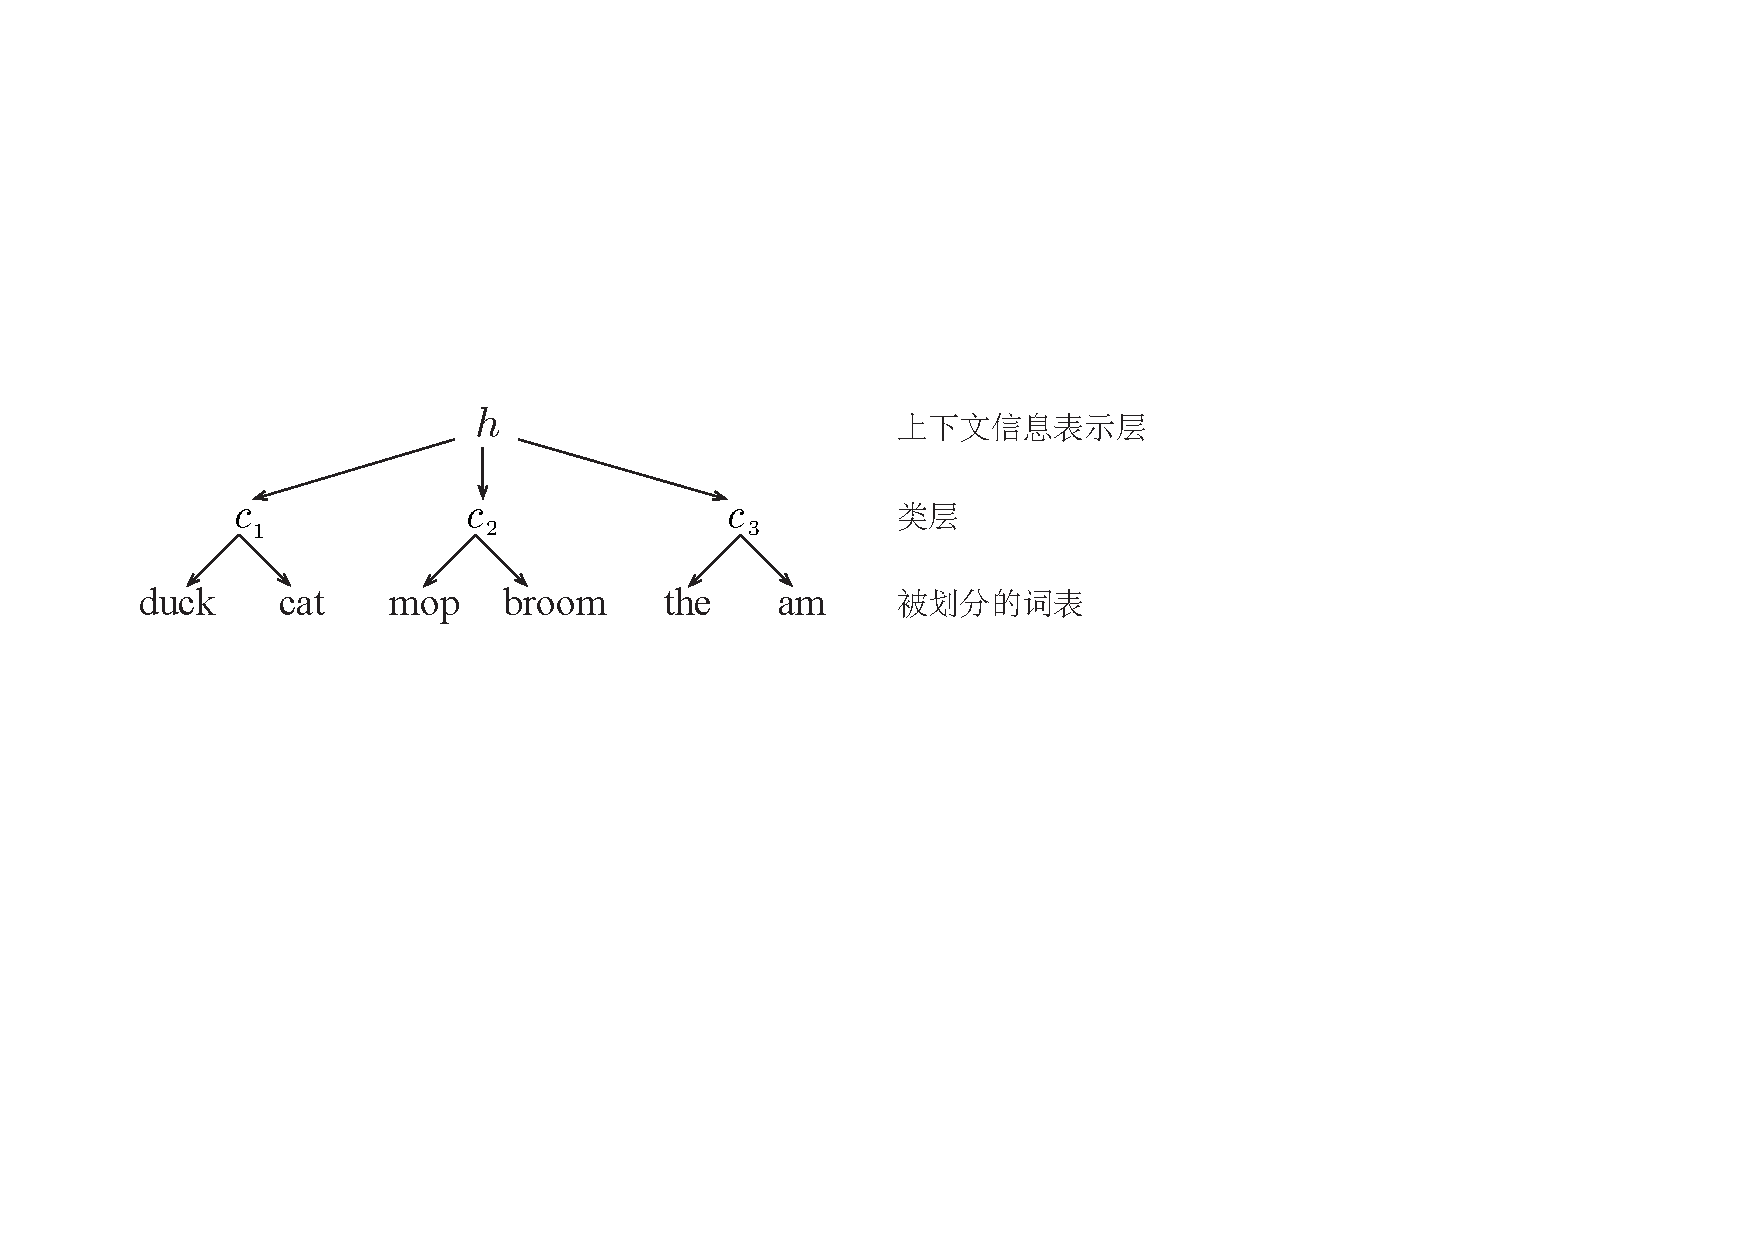
\includegraphics[width=0.7\linewidth]{./figures/case_chsm.pdf}
\caption{cHSM算法可视化模型}\label{fig:case_hsm}
\end{figure}


假设每个类包含 $\sqrt{\mathcal{|V|}}$ 单词,表示词汇被划分为相同大小的组,并且级联只涉及$2\sqrt{\mathcal{|V|}}$ 单词 softmax计算,所以最优时间复杂度可以减少到$(\mathcal{|H|}\sqrt{\mathcal{|V|}})$~\upcite{DBLP:conf/icassp/Goodman01}。虽然在更常见的情况下,分区算法会产生不同大小的字组,这需要外部努力来建立高效的数据结构并且尚未被探索。此外,精度和效率之间的权衡可以通过不同的类大小和分区算法来调整。

另一方面,tHSM方法将一步多类分类分解为多个逻辑分类步骤。正因为如此,词汇组织为二叉树,其中词在叶上,中间节点是内部参数。在平衡树结构的情况下,每个词被赋予相等长度的前缀,最优时间复杂度可以减少到$\mathcal{O}(\log \mathcal{|H||V|})$。最早的工作中,单词在二叉树上的分布可以由WordNet与人类专家~\upcite{DBLP:conf/aistats/MorinB05}或单词 unigram 分布~\upcite{DBLP:conf/nips/MikolovSCCD13}的霍夫曼编码构建。然而,在现实世界的挑战中,专家知识的构建是相当昂贵的,霍夫曼编码方案只考虑单数据统计,而单词的语境,句法或语义信息尚未被考虑和得到彻底的讨论。
\begin{figure}[!h]
  \centering
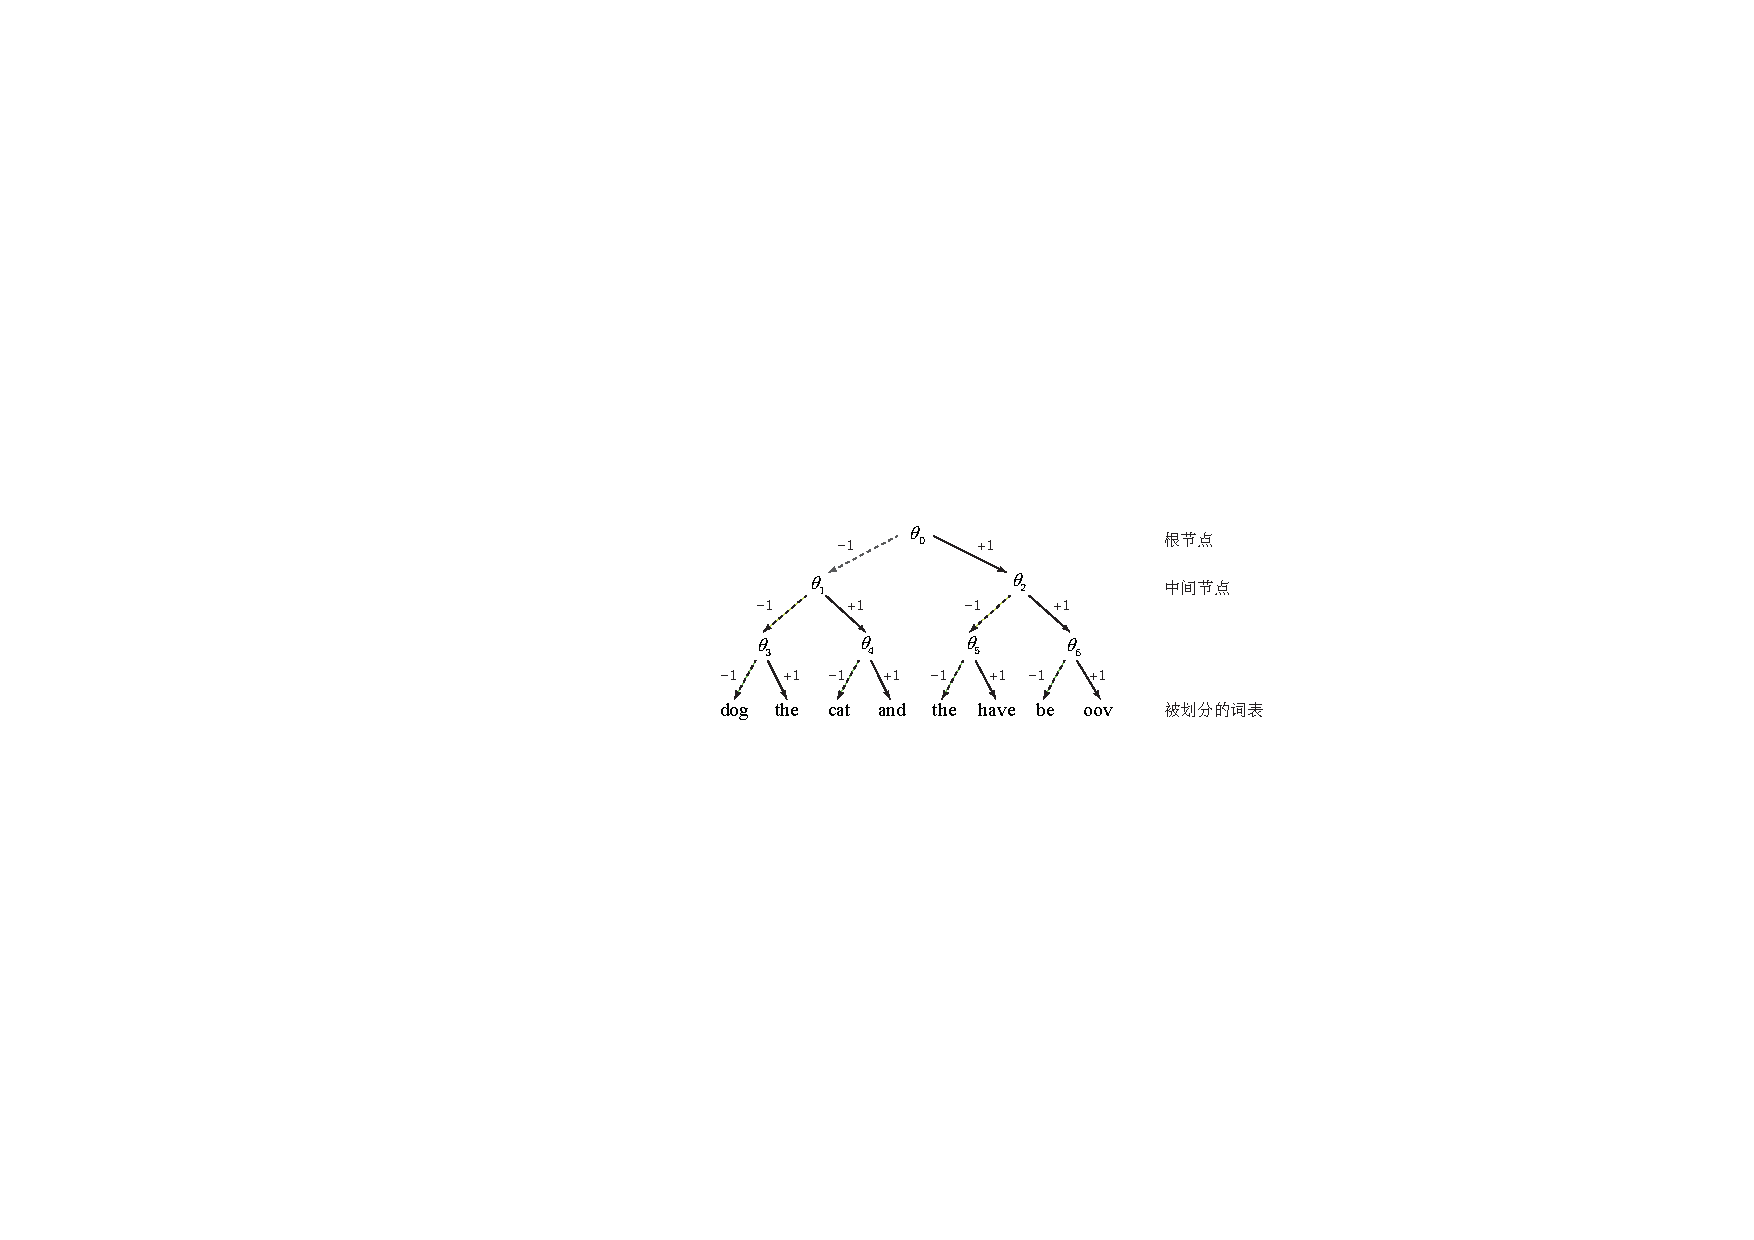
\includegraphics[width=0.9\linewidth]{./figures/thsm-example.pdf}
\caption{tHSM算法可视化模型}\label{fig:case_thsm}
\end{figure}


大词表问题,主要是对softmax如何建模的问题。在本课题中,我们探讨 cHSM 和 tHSM 两种不同的方案所带来的影响和优劣。
\section{本章小结}